%pdflatex-../thesis.tex
% vim:spell spelllang=en_us

\section{Measurement samples}
\label{appendix:measurement-samples}
% 239 
\begin{figure}[htb]
	\begin{center}
	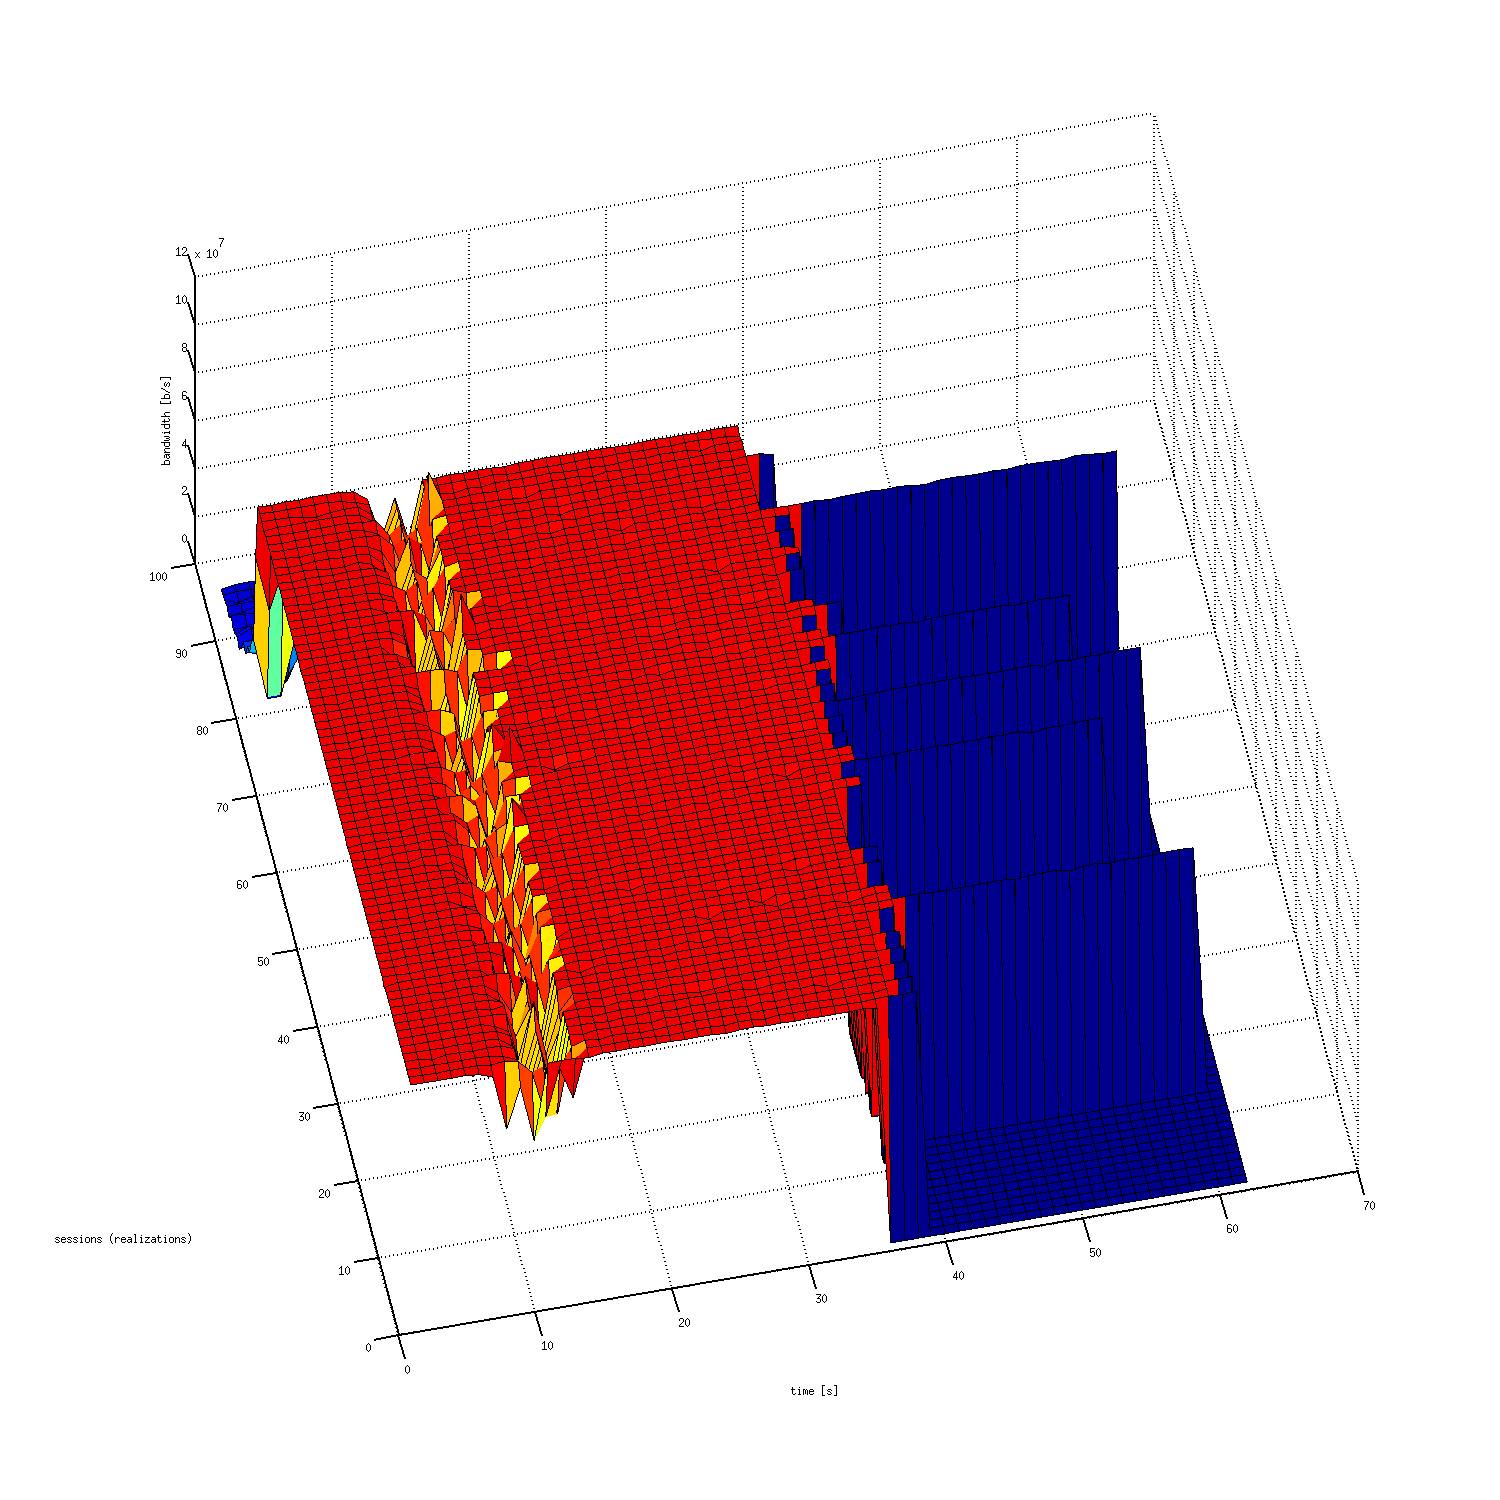
\includegraphics[width=\textwidth]{results-239-3d.png}
	\end{center}
	\caption{results-239-3d.png}
	\label{img:results-239-3d.png}
\end{figure}

\begin{figure}[htb]
	\begin{center}
	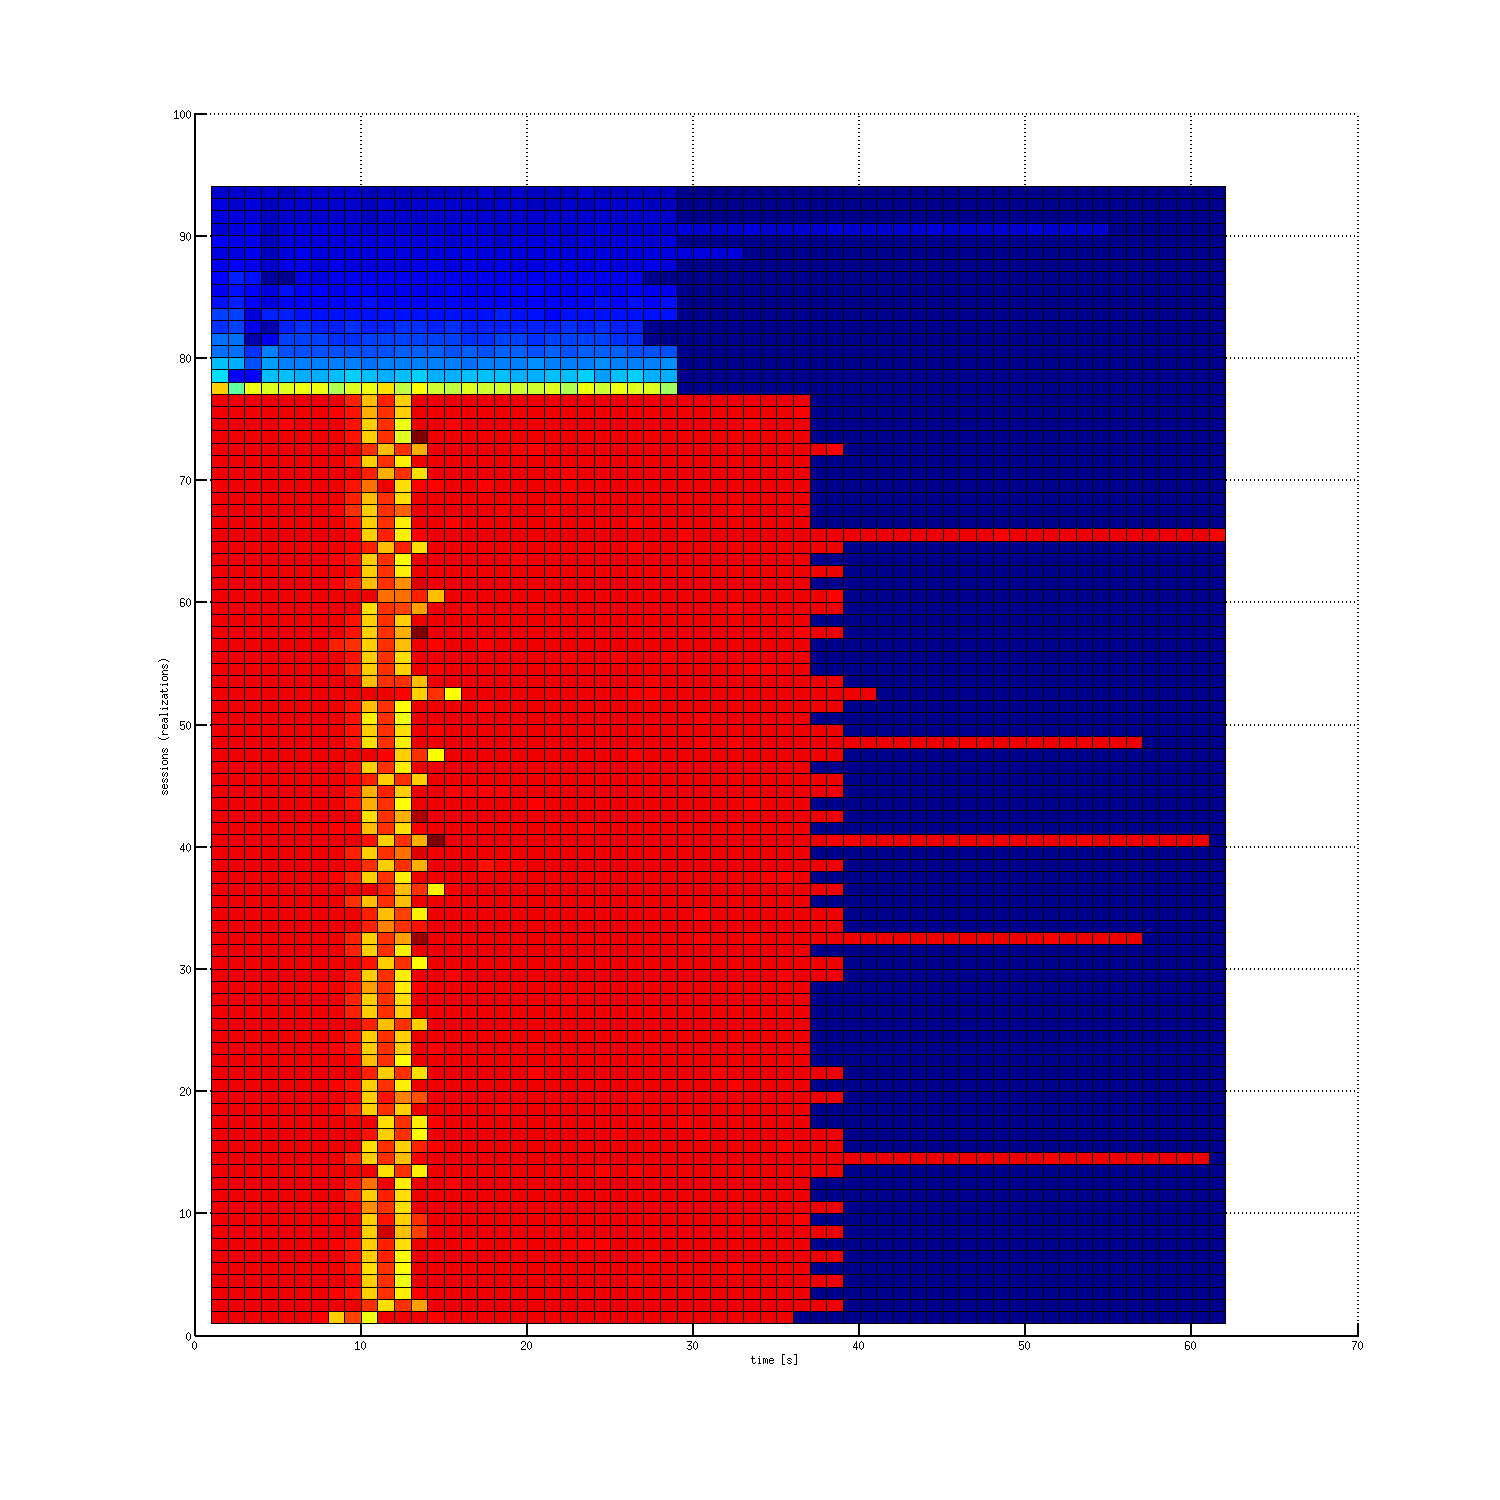
\includegraphics[width=\textwidth]{results-239-2d.png}
	\end{center}
	\caption{results-239-2d.png}
	\label{img:results-239-2d.png}
\end{figure}

% 269
\begin{figure}[htb]
	\begin{center}
	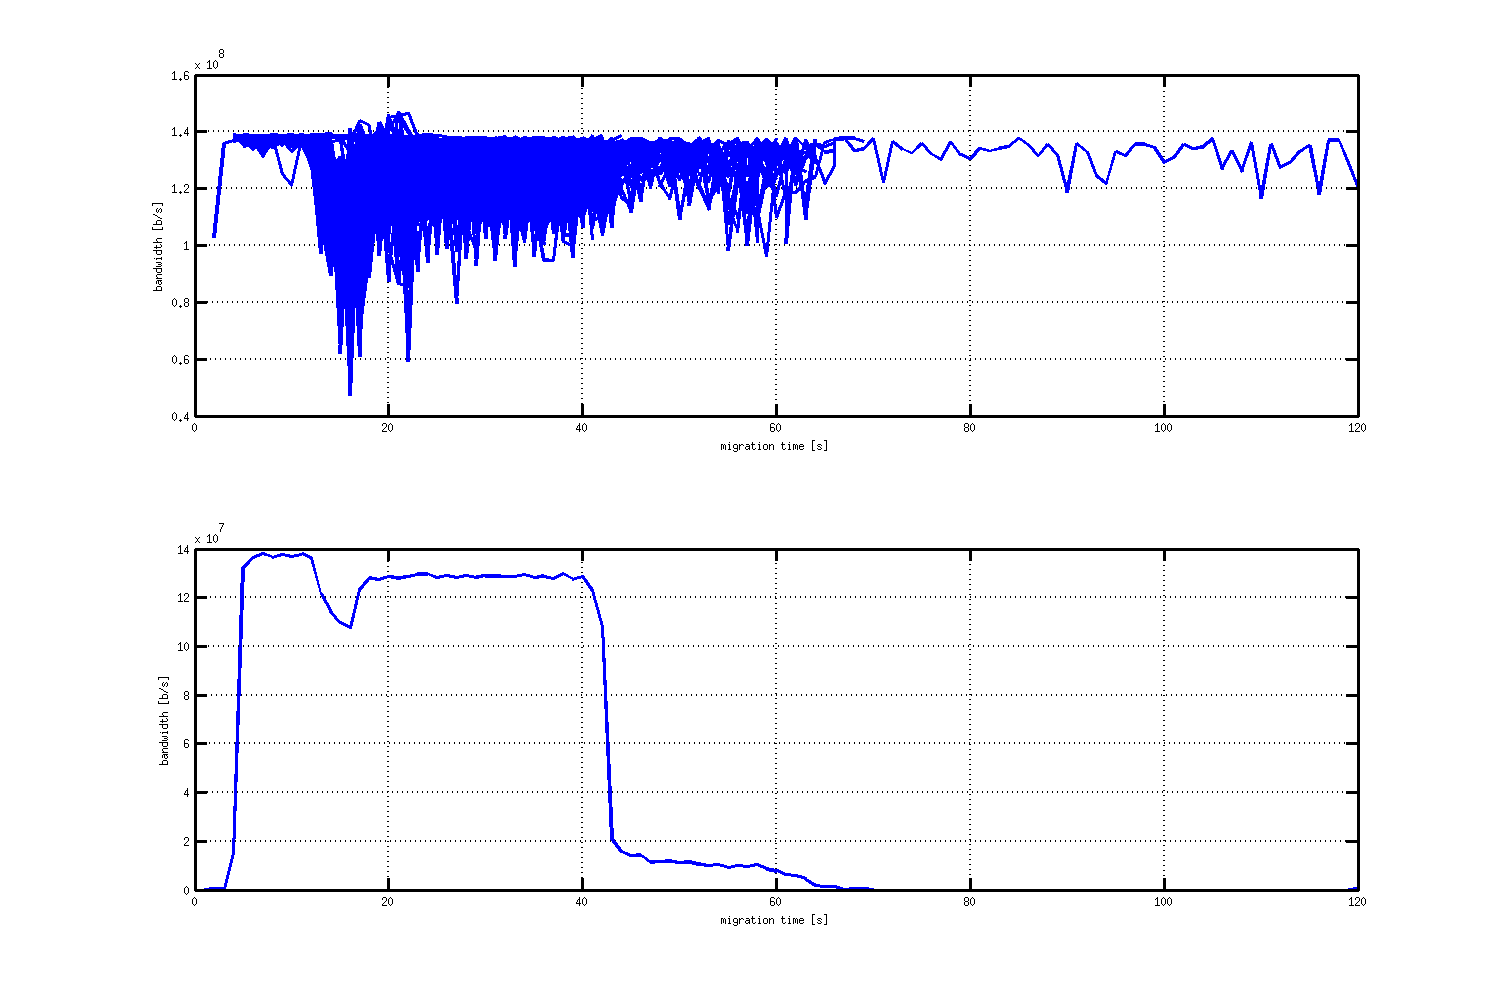
\includegraphics[width=\textwidth]{results-269-all.png}
	\end{center}
	\caption{results-269-all.png}
	\label{img:results-269-all.png}
\end{figure}
\begin{figure}[htb]
	\begin{center}
	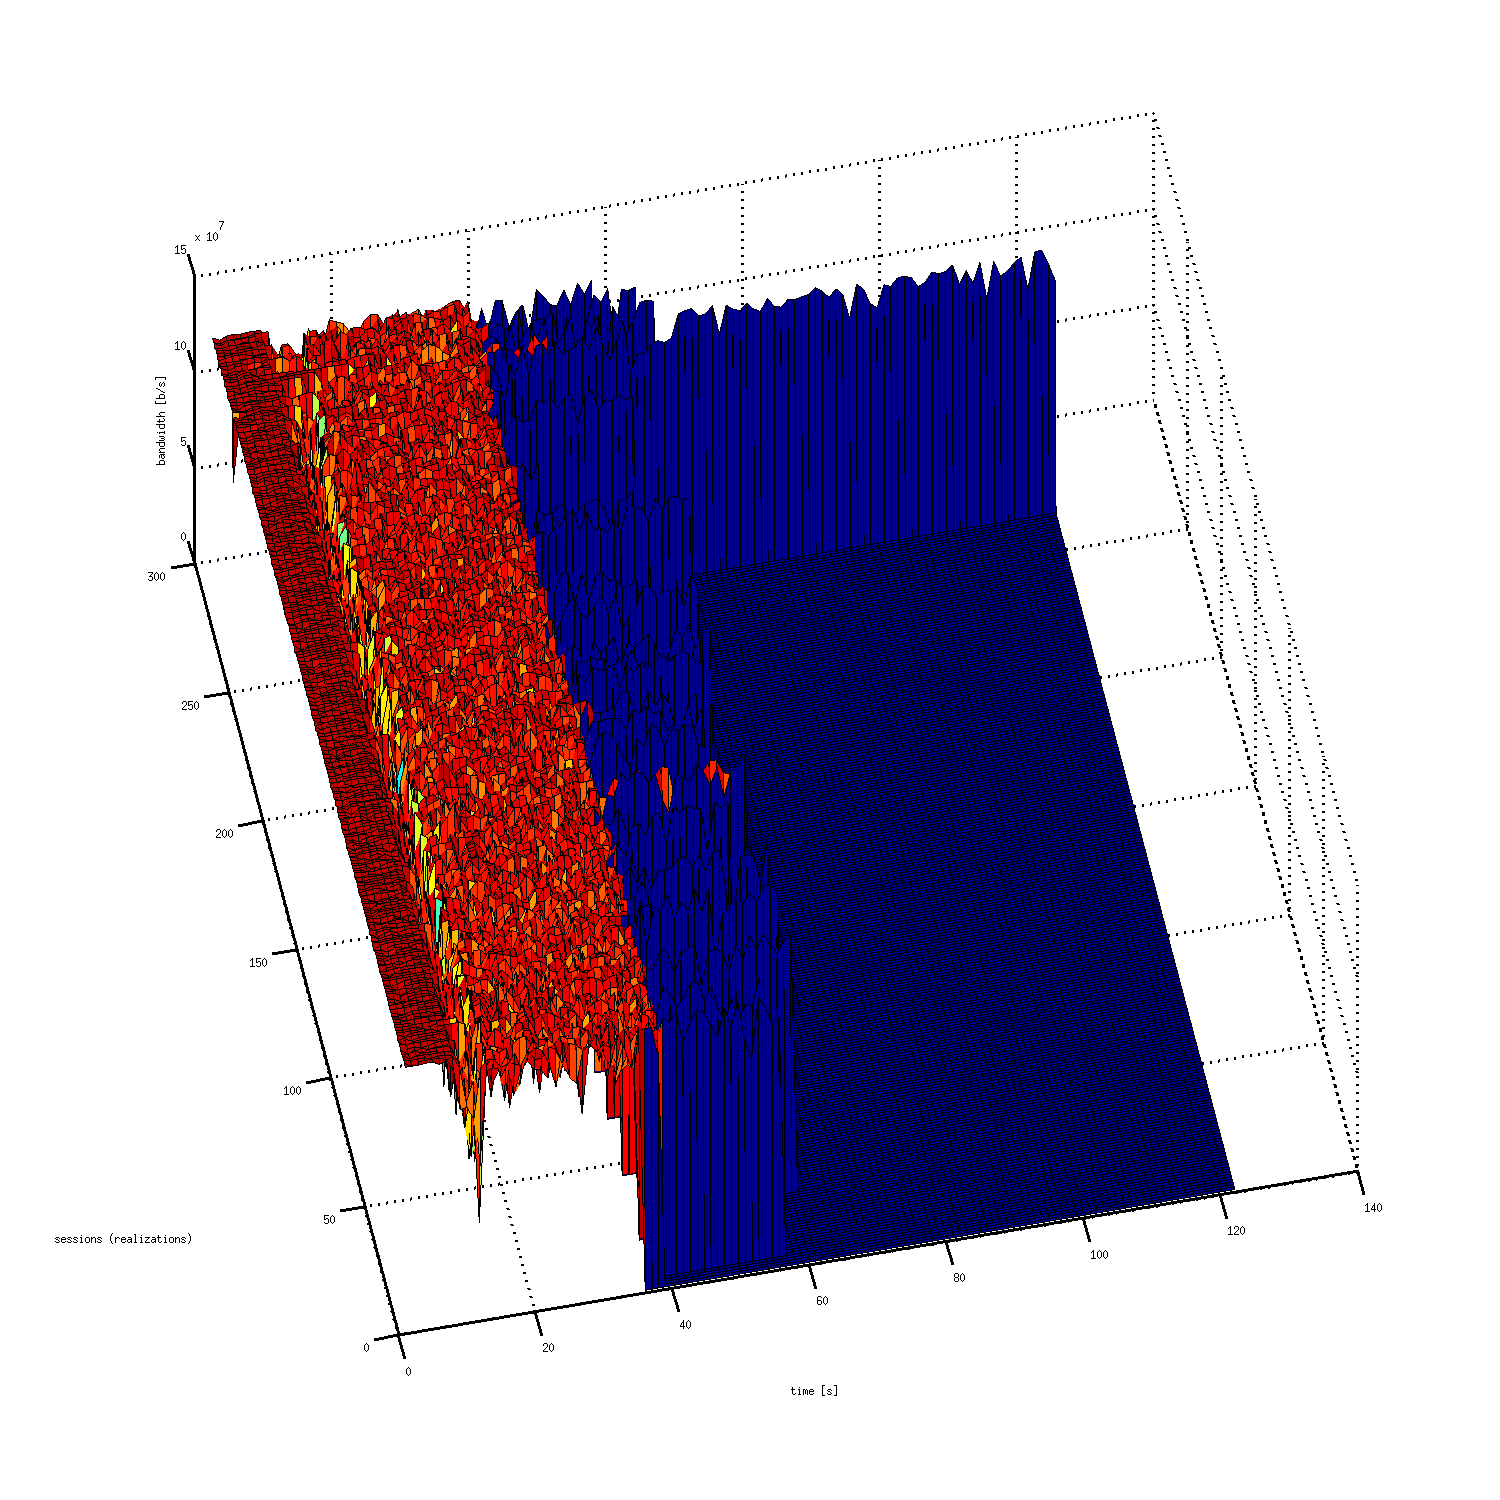
\includegraphics[width=\textwidth]{results-269-3d.png}
	\end{center}
	\caption{results-269-3d.png}
	\label{img:results-269-3d.png}
\end{figure}
\begin{figure}[htb]
	\begin{center}
	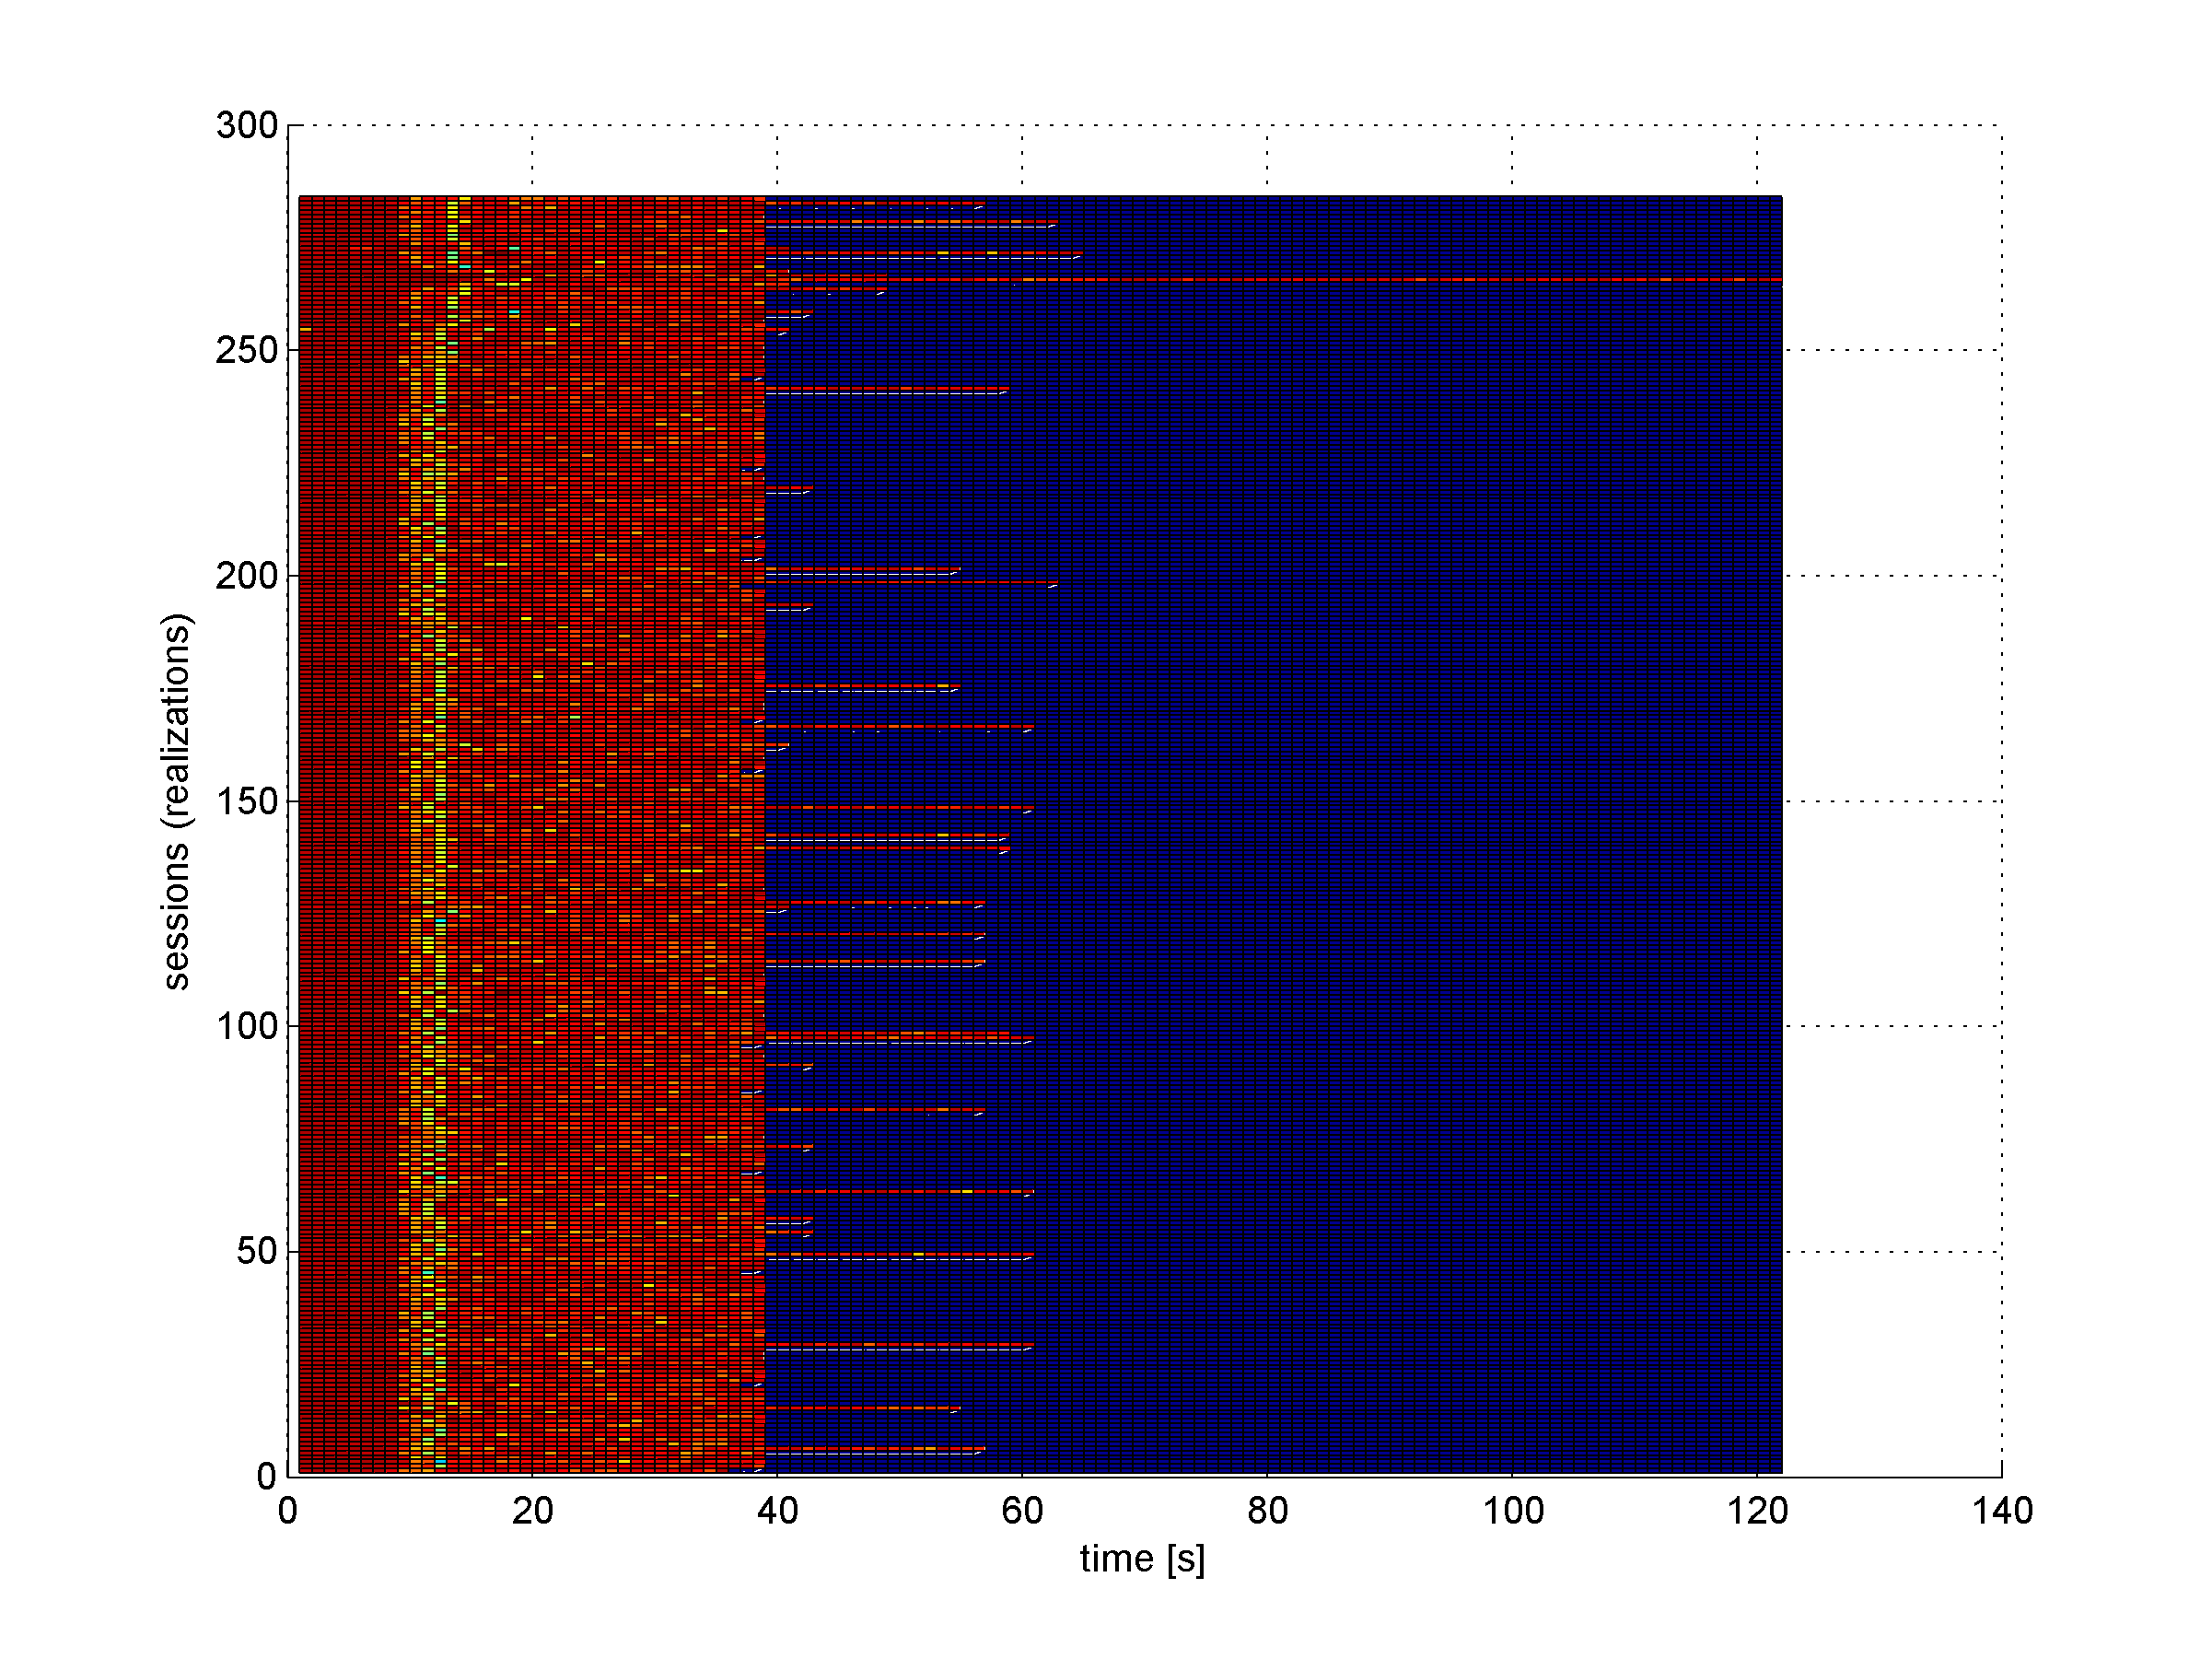
\includegraphics[width=\textwidth]{results-269-2d.png}
	\end{center}
	\caption{results-269-2d.png}
	\label{img:results-269-2d.png}
\end{figure}

% 274
\begin{figure}[htb]
	\begin{center}
	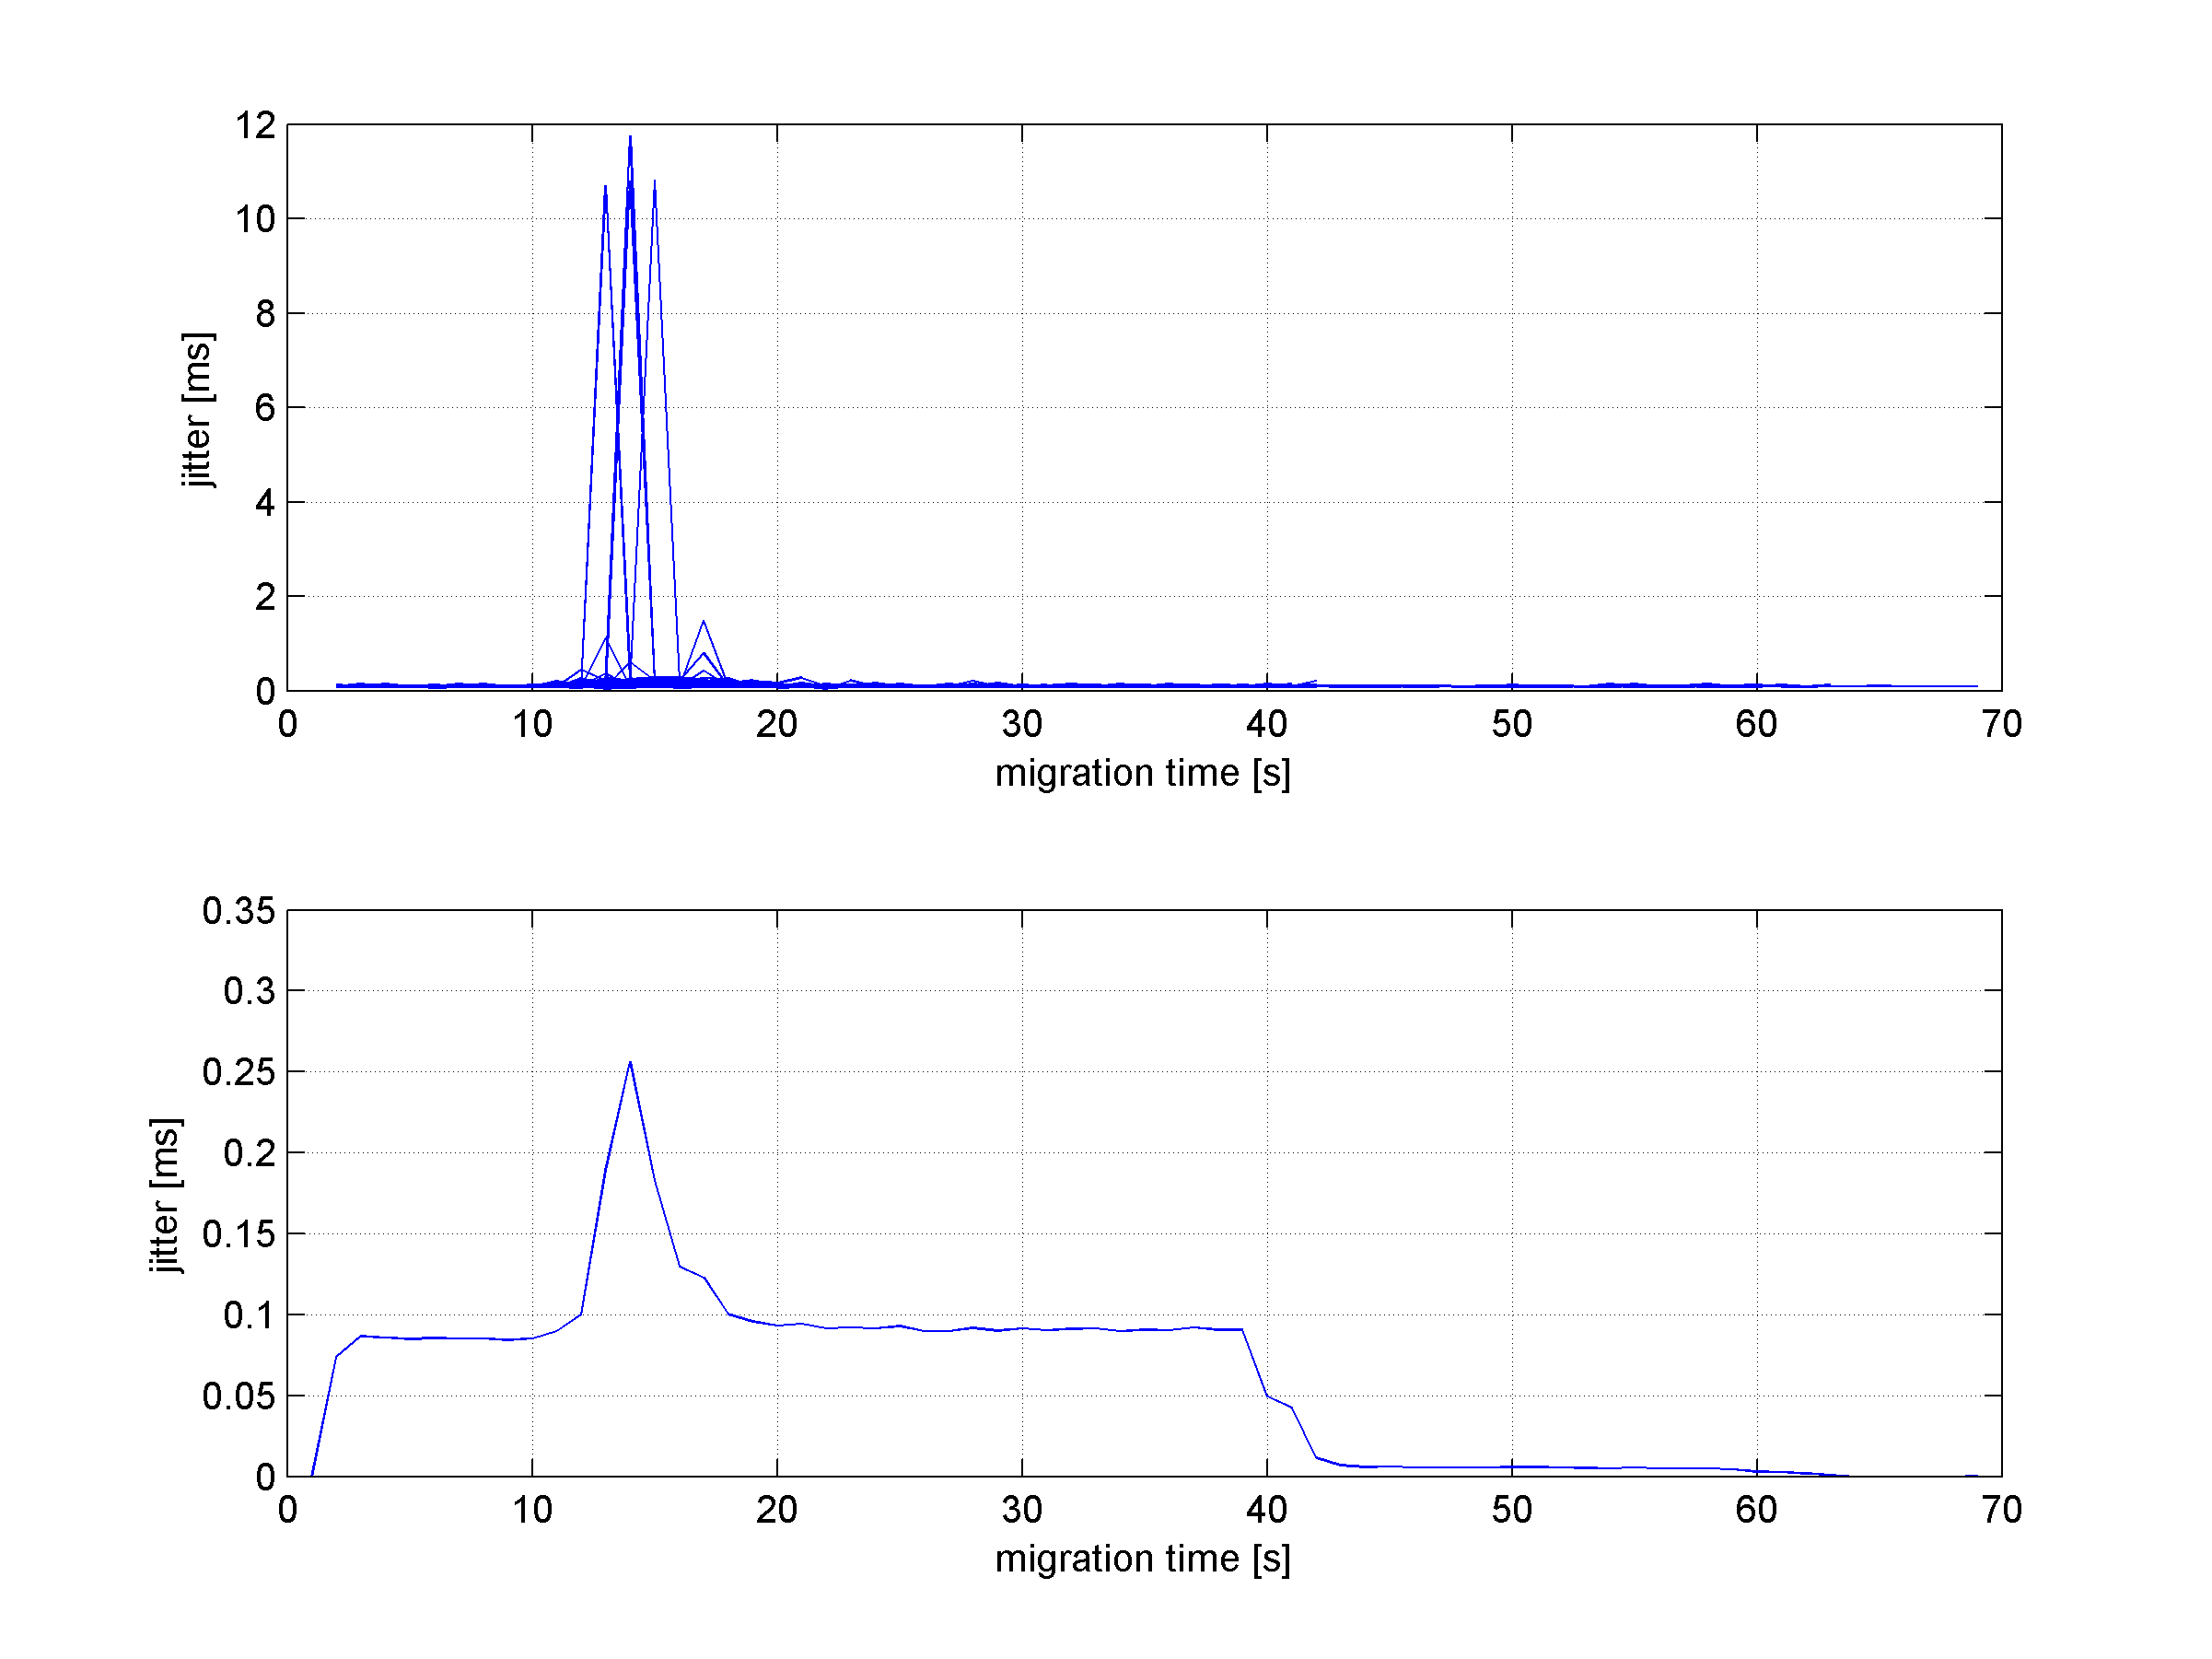
\includegraphics[width=\textwidth]{results-274-all.png}
	\end{center}
	\caption{results-274-all.png}
	\label{img:results-274-all.png}
\end{figure}
\begin{figure}[htb]
	\begin{center}
	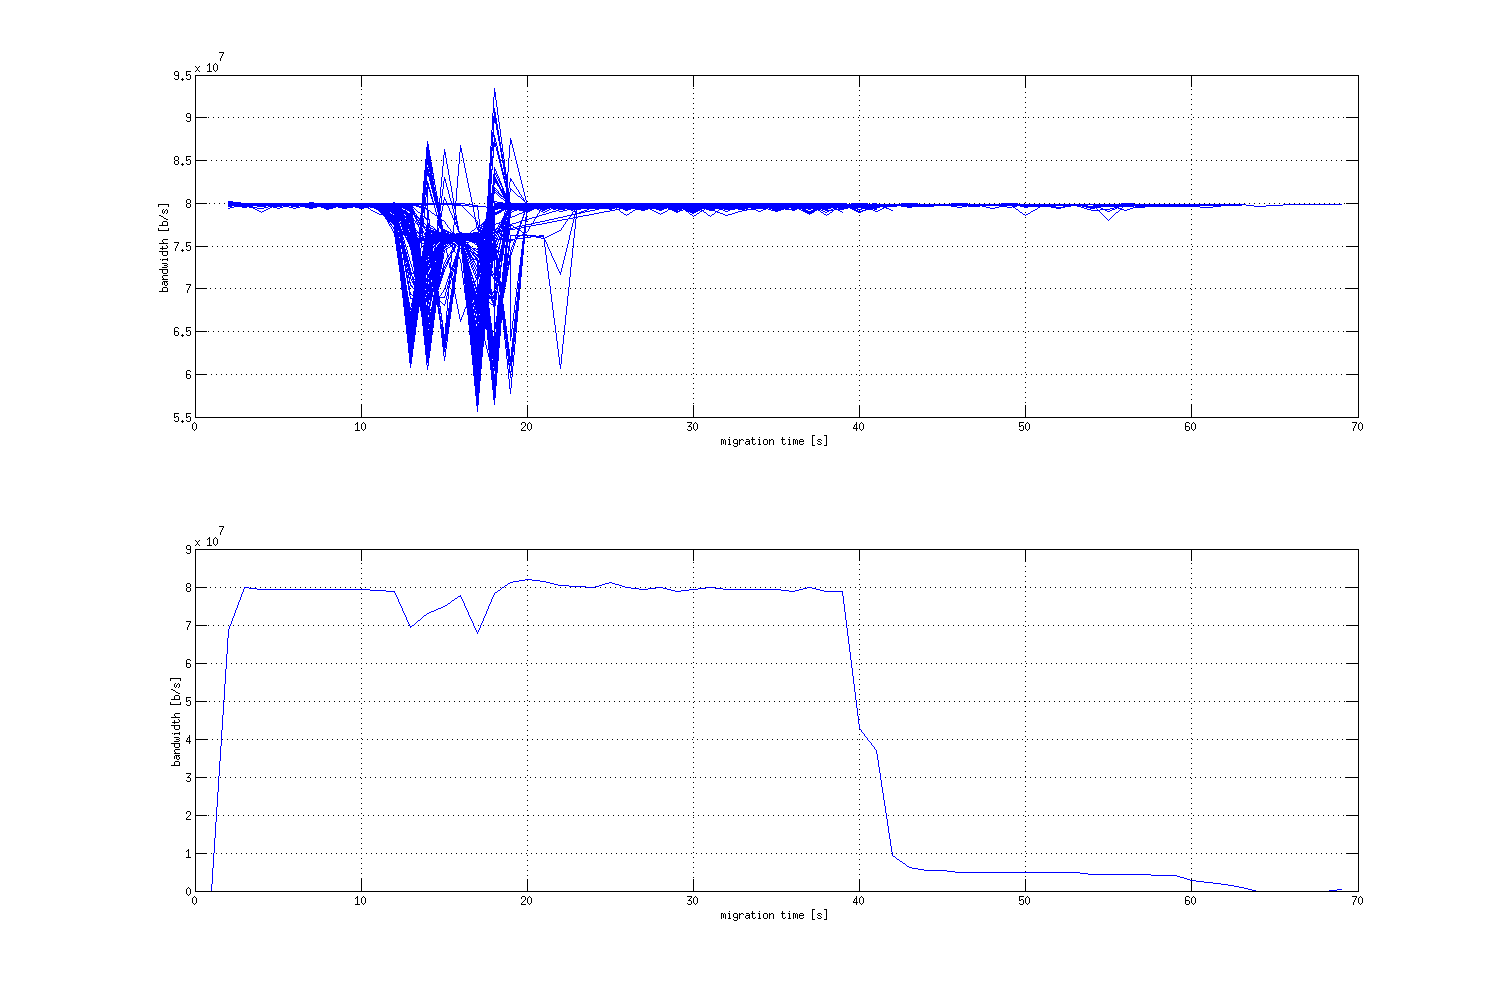
\includegraphics[width=\textwidth]{results-279-all.png}
	\end{center}
	\caption{results-279-all.png}
	\label{img:results-279-all.png}
\end{figure}
\begin{figure}[htb]
	\begin{center}
	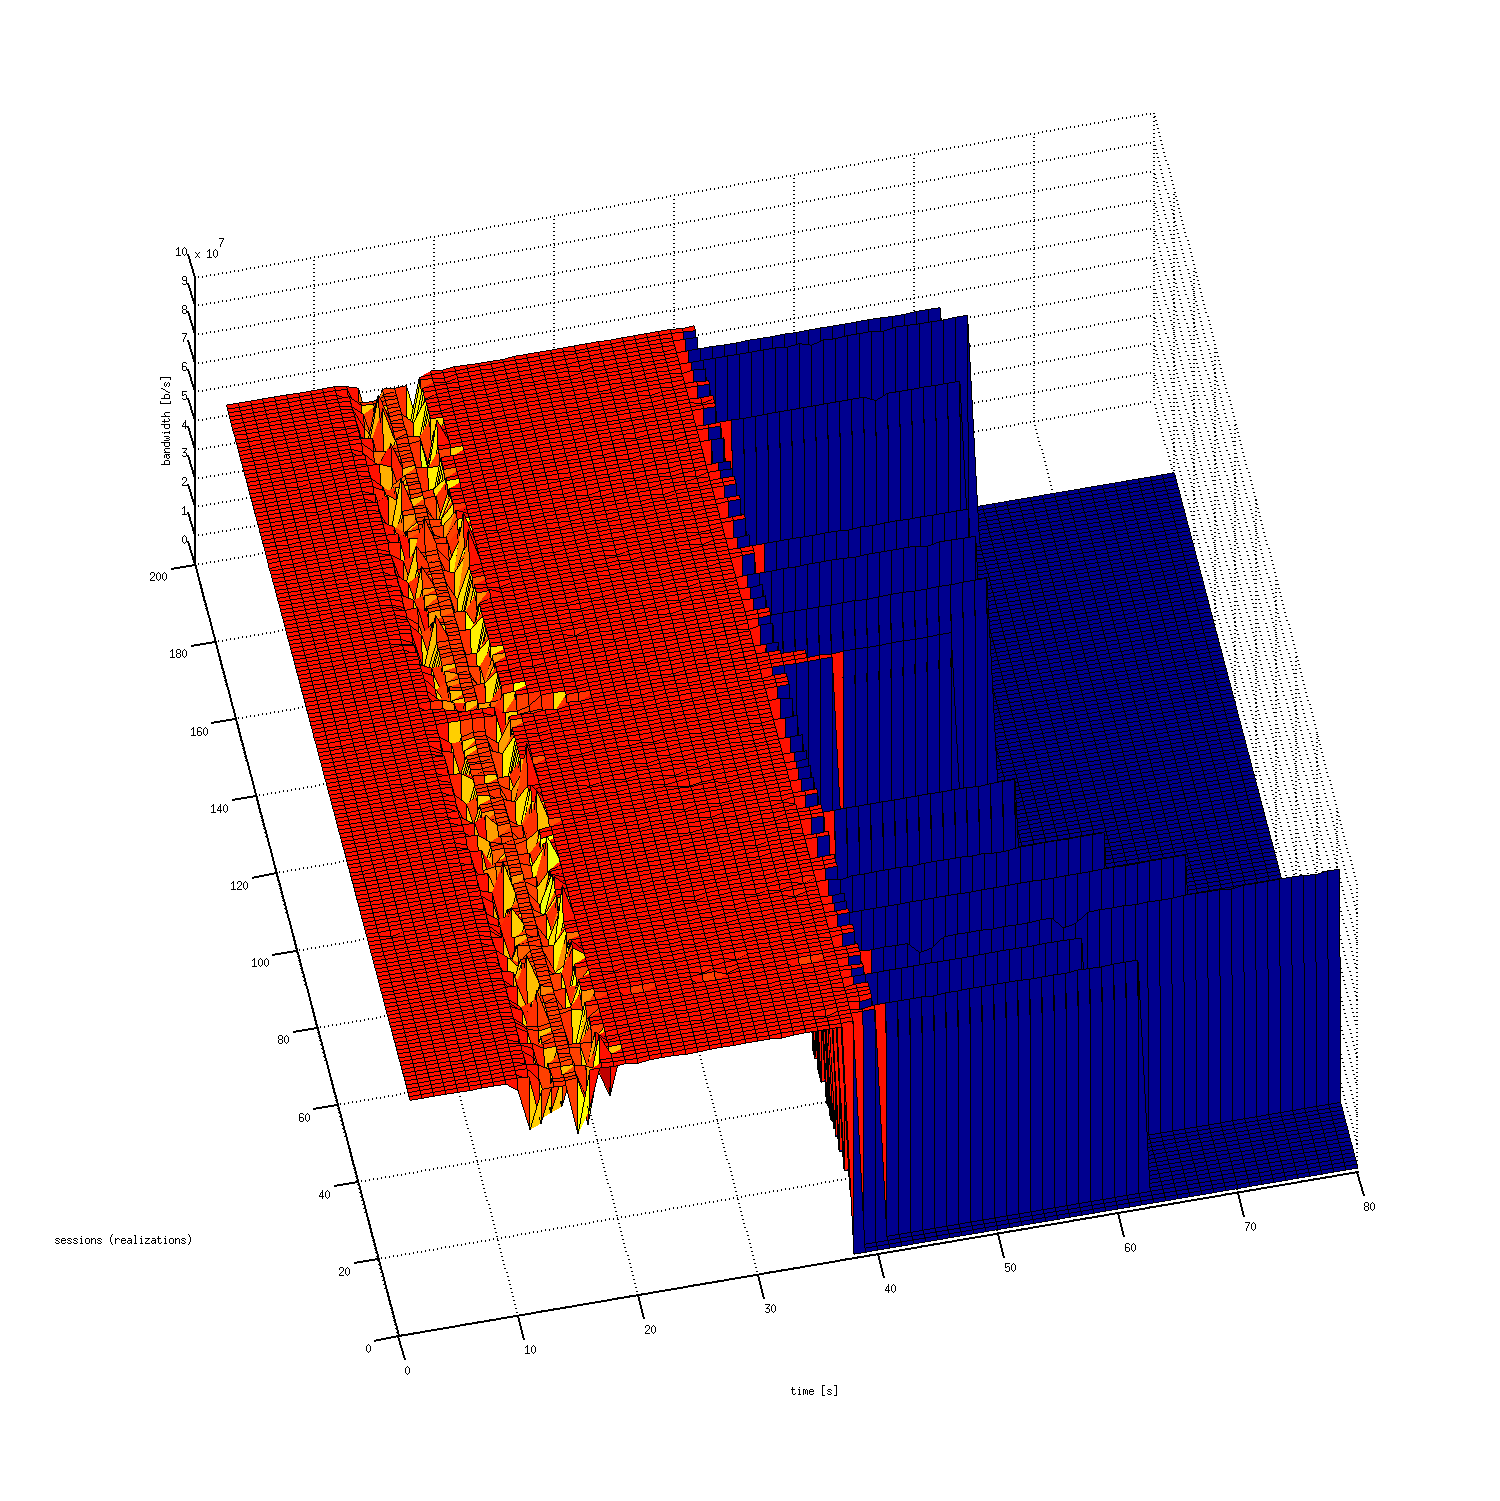
\includegraphics[width=\textwidth]{results-279-3d.png}
	\end{center}
	\caption{results-279-3d.png}
	\label{img:results-279-3d.png}
\end{figure}
\begin{figure}[htb]
	\begin{center}
	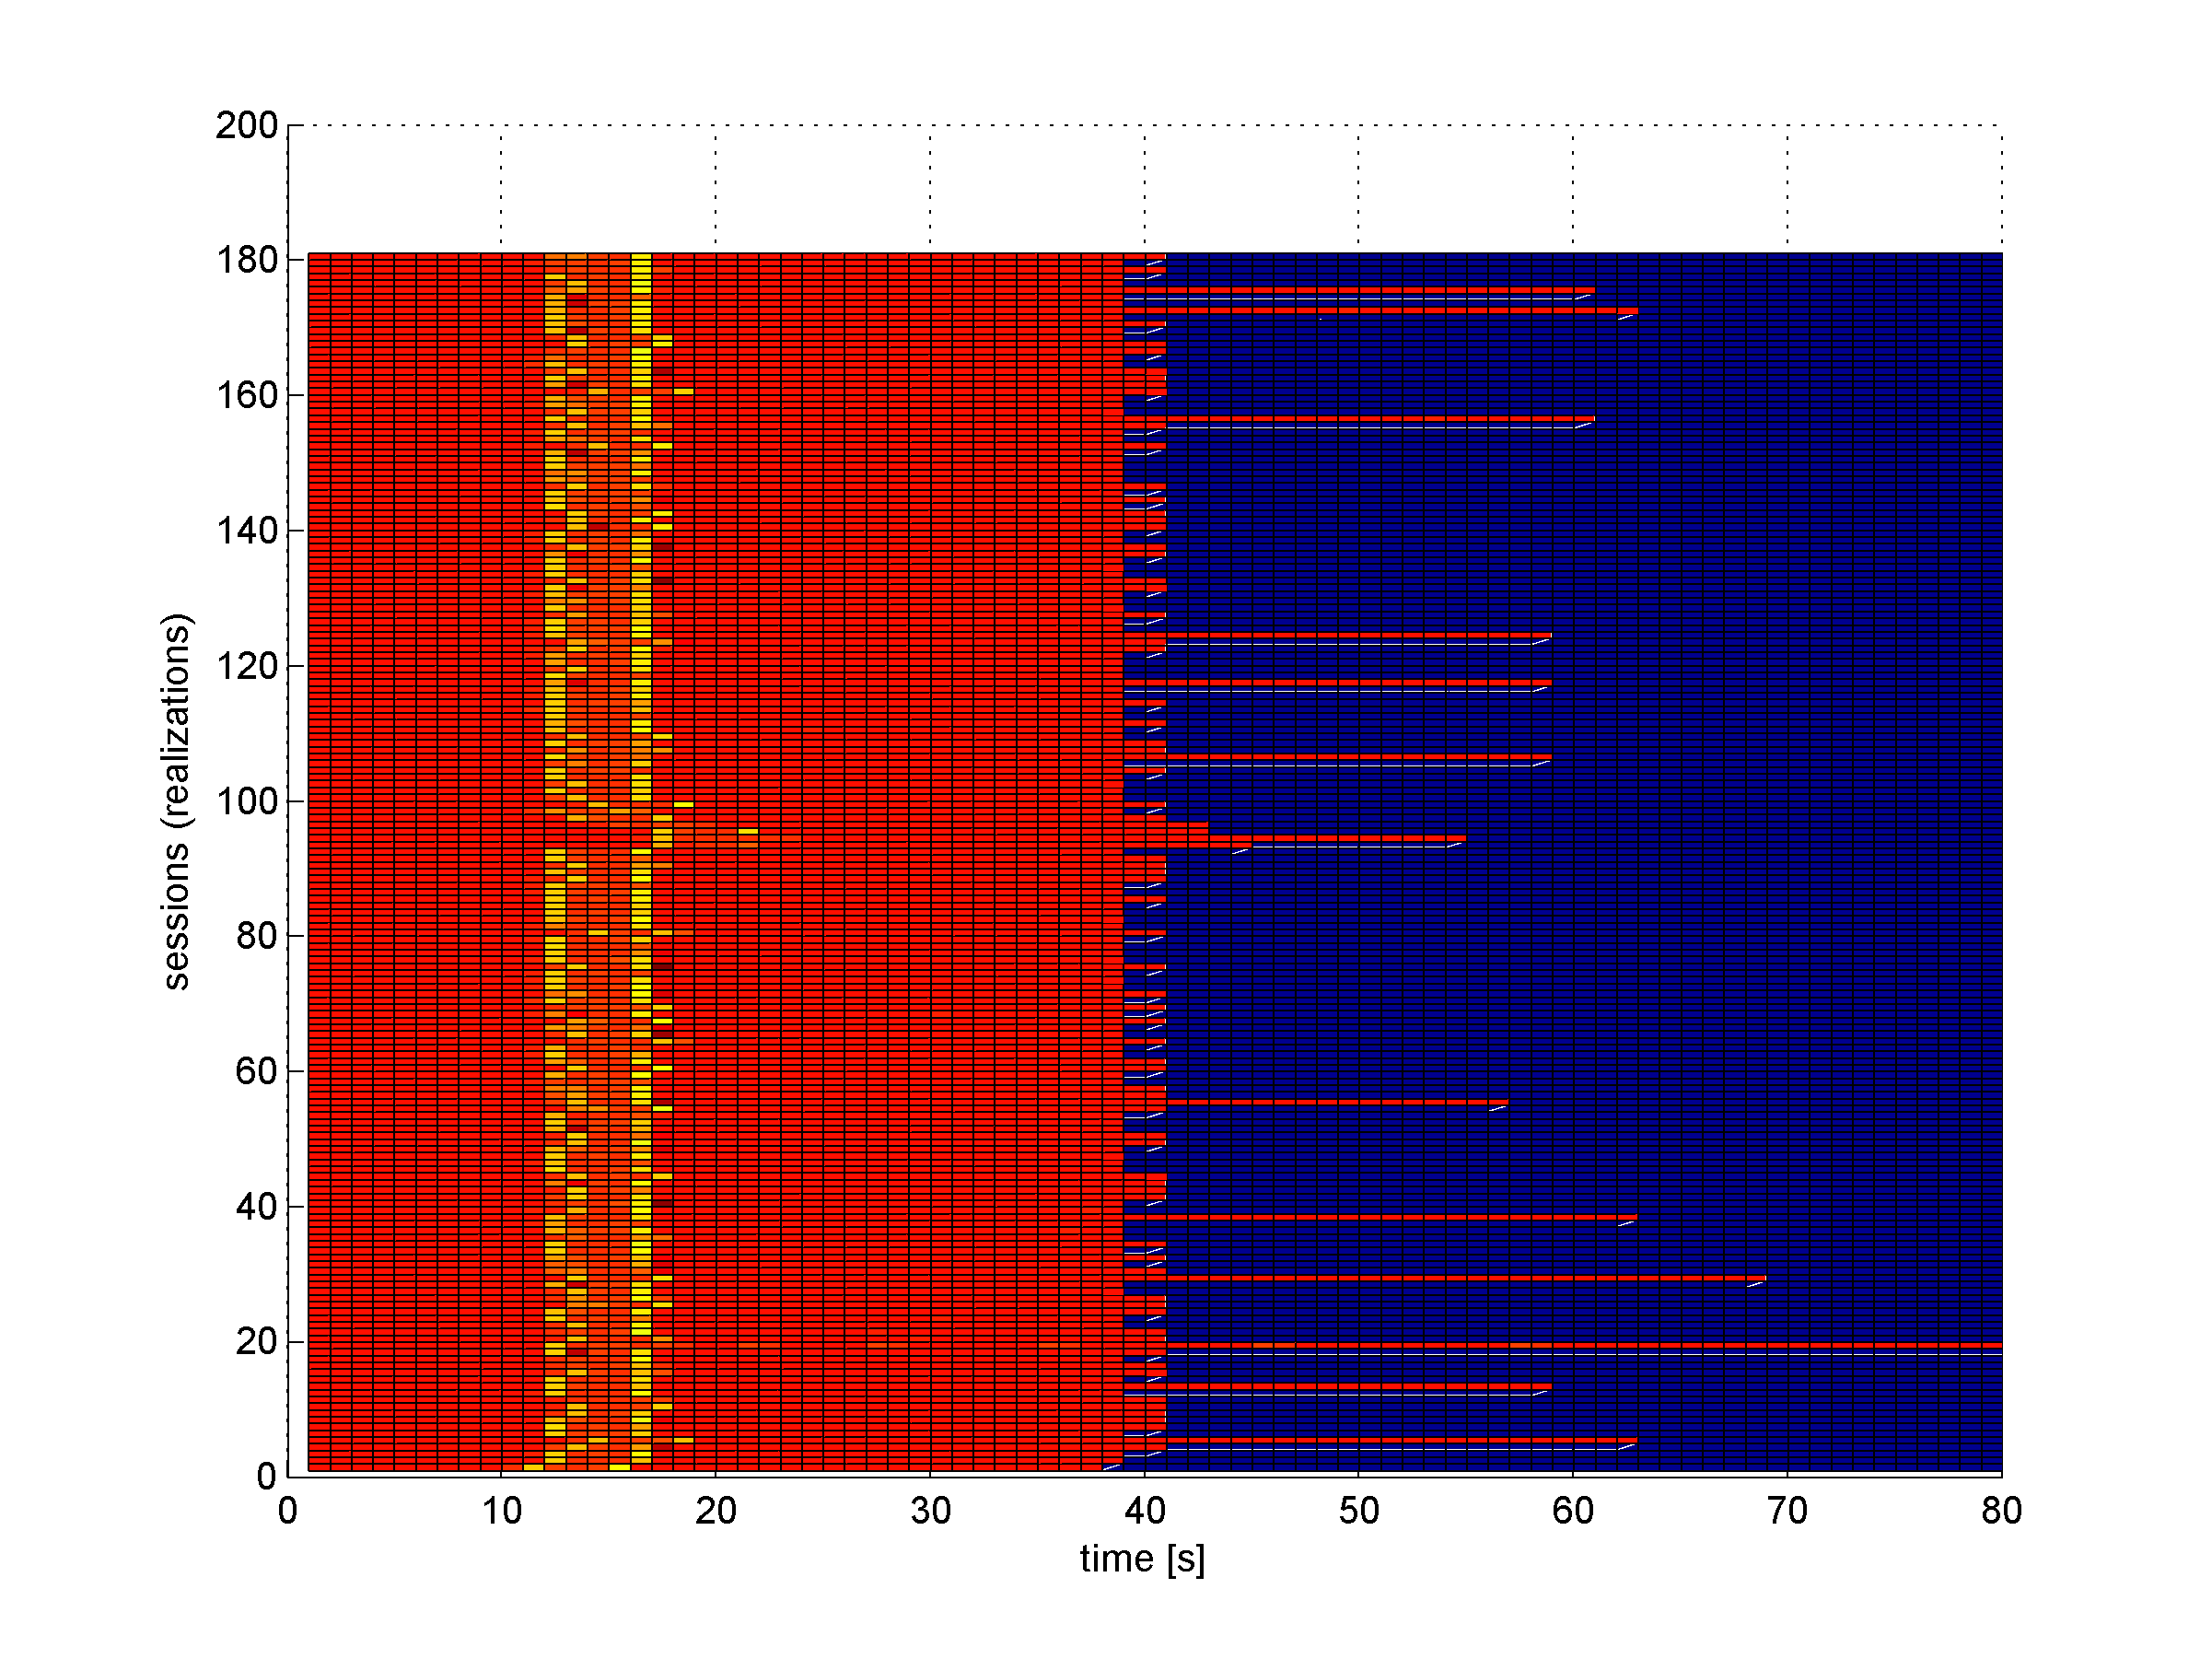
\includegraphics[width=\textwidth]{results-279-2d.png}
	\end{center}
	\caption{results-279-2d.png}
	\label{img:results-279-2d.png}
\end{figure}

